\documentclass[twoside,letterpaper,twocolumn]{article}

%%%%%%%%%%%%%%%%%%%%%%%%%%%%%%%%%%%%%%%%%%%%%%%%%%%%%%%%%%%%%%%%%%%%%%
% Package with format specifications for the 9th CISBGf
\usepackage{cisbgf}
\usepackage{booktabs} 


%%%%%%%%%%%%%%%%%%%%%%%%%%%%%%%%%%%%%%%%%%%%%%%%%%%%%%%%%%%%%%%%%%%%%%
% MANDATORY PARAMETERS

% Setting the title
\title{Analysis of Crustal Structure in the region of Ribeira Belt (between the Provinces of the S\~{a}o Francisco Craton and the Paran\'{a} Basin) using Seismological Methods.}  

% Setting the authors
\author{Diogo Luiz de Oliveira Coelho, St\'{e}phane Drouet, Observat\'{o}rio Nacional, Rio de Janeiro, Brazil
}

% Setting the headings
\headauthor{Coelho and Drouet}
\headtitle{Analysis of Crustal Structure using Seismological Methods}


%%%%%%%%%%%%%%%%%%%%%%%%%%%%%%%%%%%%%%%%%%%%%%%%%%%%%%%%%%%%%%%%%%%%%%
%%%%%%%%%%%%%%%%%%%%%%%%%%%%%%%%%%%%%%%%%%%%%%%%%%%%%%%%%%%%%%%%%%%%%%
\begin{document}

\maketitle

\begin{abstract}

The work area covering the north of S\~{a}o Paulo, South of Rio de Janeiro e South of Minas Gerais. Our study have as main goal generate images of crustal discontinuities. With these images we intend add information about the local geological framework, corroborating for delineate with accuracy the discontinuities. Were installed twenty four seismograph stations in three sections, two perpendiculars to coast and one parallel. The distance between the stations  is approximately 20 km.
The first analysis done is noise level and to calculate a regional crustal thickness was used the method called Receiver Function. To obtain a image of discontinuities, as Moho, the stacking of Receiver Functions are mapped in relation to station position in the section. The calculated values of the Moho depth for each station were linearly interpolated to generate a regional map. We see the Moho thinning in direction to east, reinforcing the proximity with the oceanic crust.

\end{abstract}

\section{Introduction}

The work area is found in the geographic quadrant sited between the coordenates north (21°19’5” S/45°39’31” W e 22°7’59” S/46°54’23” W) and south (23°8’28” S/48°13’28” and 23°57’33” S/45°28’35” W) covering the north of S\~{a}o Paulo, South of Rio de Janeiro e South of Minas Gerais. Localized near the cities like: Parati-RJ; Guaratinguet\'{a}-SP; Taubat\'{e}-SP; Ubatuba-SP; S\~{a}o Jos\'{e} dos Campos-SP; Caraguatatuba-SP; S\~{a}o Gon\c{c}alo do Sapuca\'{i}-MG; Itajub\'{a}-MG; Alfenas-MG; Varginha-MG; Pouso Alegre-MG. 
The Total area of this project is the approximately 33600 km$^{2}$.

The study area is enframed geologically in  Continental Rift of the Southeast of Brazil over polycyclic terrains referable to south of the Ribeira Belt, as \cite{riccomini_o_1990} cites in your paper. This Belt is compound for metamorphic rocks, migmatites and granitoids related to Brasiliano Orogenetic Cycle. This geological zone is titled for \cite{almeida_origem_1998} as Planalto Atlantico. The area is found on a region reworked by preterite orogenic cycles and the lithological set was intruded by transcorrents thrust systems oriented according to regional trend, direction ENE to EW, in accordance with \cite{hasui_evolucao_1976}.

The main goal is generate images of the crustal discontinuities. With these images, we intend add information about the local geological framework, corroborating for delineate with accuracy the discontinuities.


\section{Methodology}

Were installed twenty four seismograph stations in three sections, two perpendiculars to coast and one parallel, as observed in Figure \ref{figura1}. The section 1 extends from the STA01 station, located near the coast, to STA09. The section 2 goes of station STA10, north, to station STA16, near the coast. Section 3 extends from station STA17, west, to station STA24, east. The distance between the stations  is approximately 20 km.


\begin{figure}[!ht]
\centering
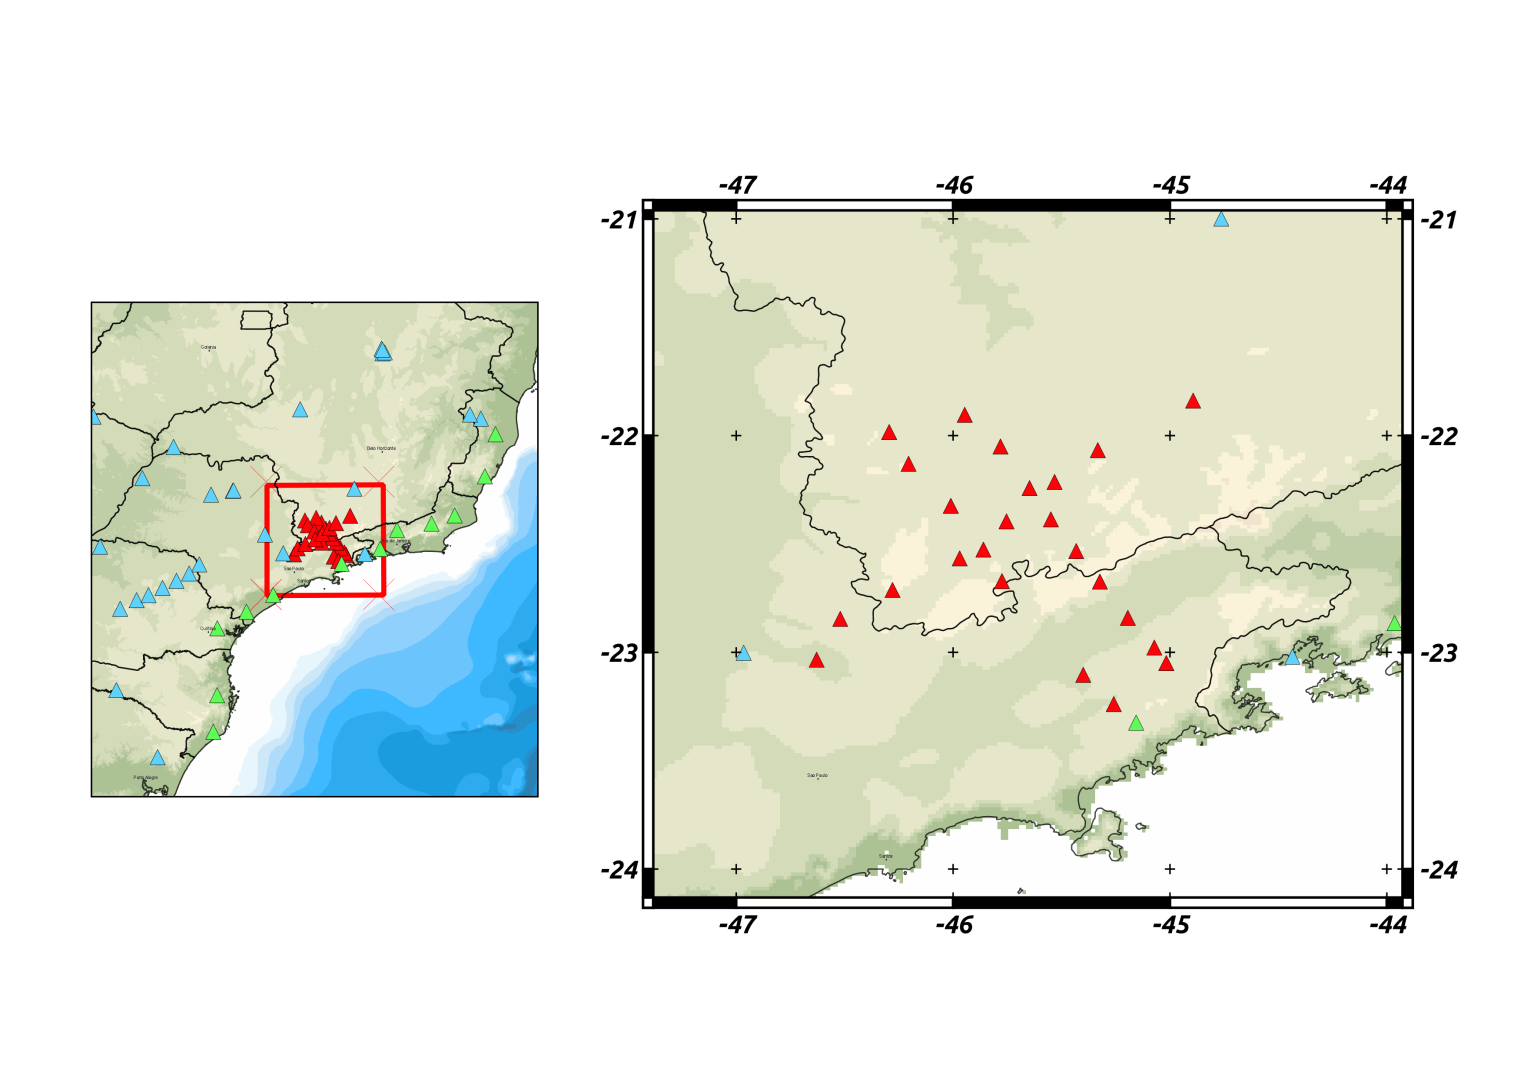
\includegraphics[scale=0.5]{mapa_das_estacoes_simosgraficas_instaladas.png}
\caption{Map of the seismograph stations installed (red triangles). The others triangles are of the Brazilian Seismographic Net.}
\label{figura1}
\end{figure}


The seismographs are broadband (STS2 ou Reftek RT151-120s) and the record frequency band is at interval 50 Hz - 100 seconds. The perpendicular sections were installed in half of 2012 and parallel section in the end of 2012. The stations ran until the end of 2013 registering the terrain movement.

The first analysis done was the mensuration of noise level in the stations using PQLX software. The calculus of noise level is based in the work of \cite{mcnamara_ambient_2004}. The data was separated in intervals of one hour with 50\% of superposition. Each interval was separated in 13 parts with 75\% of superposition to calcule a "Power Spectral Density”. Later was partitioned in 13 parts with 75\% of superposition to calculate a "Power Spectral Density”. The obtained means for each one of 13 parts are used to estimate a "Probability Density Functions” that are estimates by the calculus of the means for the total number of hourly interval.

This method differs of others utilized because is not necessary display the data to remove the existing noise. The noise is compound by calibration seisms, cultural noise, instrumental problems and a lack of data. These types of noise have a low Probability Density Functions, according \cite{mcnamara_ambient_2004}, then is suppressed.

To calculate a regional crustal thickness was used the method called Receiver Function, that was developed for \cite{langston_effect_1977}. That method use the signal of teleseisms, generators of plane waves of quasi-vertical incidence beneath a given station. The P wave arrival in the Mohorovicic seismic discontinuity, also known as Moho, and decomposes in a transmitted P wave e a converted S wave. The difference of arrival time of both waves and of others reflections allows infer Moho thickness, as observed in the Figure \ref{figura2}.

\begin{figure}[!ht]
\centering
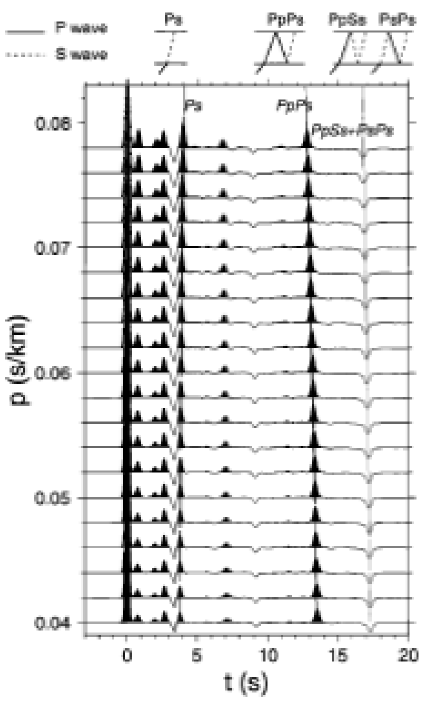
\includegraphics[scale=1.3]{funcoes_do_receptor.png} \caption{Synthetic Receiver Fuction} \citep{zhu_moho_2000}
\label{figura2}
\end{figure}
 
Seisms near of station, distance less than 20 degrees, generate waves with oblique incidence and this data type should be utilized with careful. In seisms with distances bigger than 95 degrees, the P waves don't arrive in station due to  the velocity inversion in the mantle-core boundary. Another important fact is that cannot observed a direct P wave.

The Receiver Functions are calculated with a deconvolution in time-domain of the radial component by the vertical component. This eliminates similar parts of signals, source and source's propagation until Moho. The Receiver Function is sensible in the delimitation of crustal superficial structuration under the station. The software SAC (\textit{Seismic Analysis Code}) was used to process and to calculate the Receiver Functions. 

A robust method to analyse the Receiver Functions is the method of \cite{zhu_moho_2000}. Using the medians velocities in the crust, the time differences between P wave and a converted P wave in S can be calculated, as well as the time of multiples.

\begin{eqnarray}
H &=& \frac{t_{P_{s}}}{\sqrt{\frac{1}{v_{s}^{2}}-p^{2}}-\sqrt{s\frac{1}{v_{p}^{2}}-p^{2}}}
\\
H &=& \frac{t_{P_{p}P_{s}}}{\sqrt{\frac{1}{v_{s}^{2}}-p^{2}}+\sqrt{\frac{1}{v_{p}^{2}}-p^{2}}}
\\
H &=& \frac{t_{P_{p}S_{s}}+t_{P_{s}P_{s}}}{2\sqrt{\frac{1}{v_{s}^{2}}-p^{2}}}
\end{eqnarray}

Using a given velocity  $v_{p}$, the arrival times can be calculate with the Moho thickness(H), the $v_{p}/v_{s}$ ratio and the ray parameter, this depends of location and depth of the event. Rather than trying to adjust all the function, the method make a search,\textit{grid search}, of the crustal thickness and the $v_{p}/v_{s}$ ratio to calculate the theoretical arrival times of the converted P waves in S and your multiples for each register. The best combination of crustal thickness and $v_{p}/v_{s}$ ratio is one that maximizes the value of the real amplitudes of the Receiver Functions.

To obtain a image of discontinuities, as Moho, the stacking of Receiver Functions are mapped in relation to station position in the section. The data are divided in 4 groups, according the azimuth between the seism and the station. The majority of the events occur in the northwest and southwest region, we can note a scarcity of quakes in the region of Atlantic Ocean. The goal of this separation is evaluate if exist lateral variation of structure.

\section{Results}

The Figure \ref{figura3} shows the registered events in STA08 station. The most part of seisms recorded in stations are events from Andes range or Central America.

\begin{figure}[!ht]
\centering
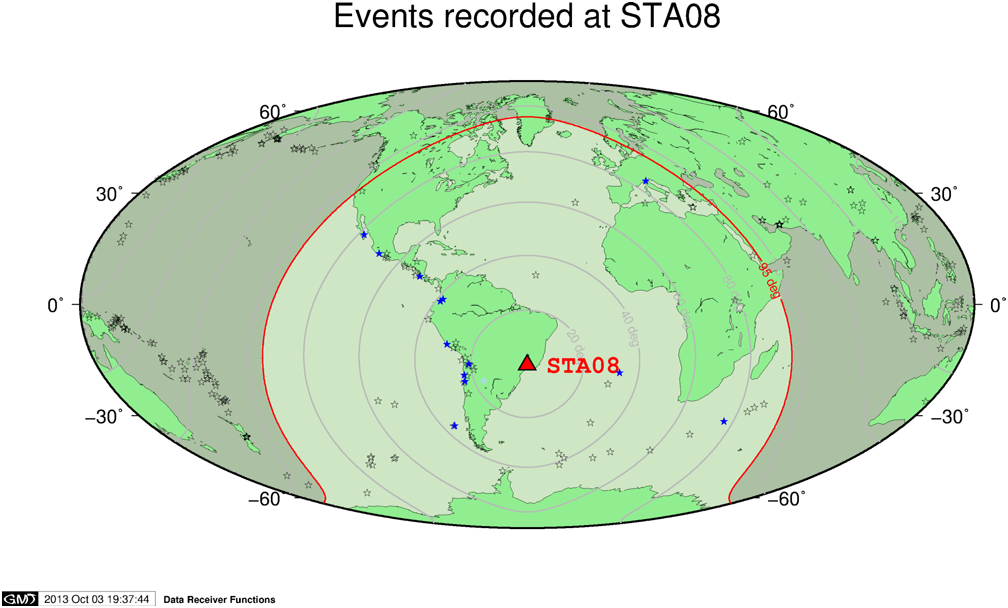
\includegraphics[scale=0.48]{mapa_de_eventos.png} \caption{Map with recorded events by STA08 station. The red triangle represents the station and the blue stars represent the seisms.} 
\label{figura3}
\end{figure}
 
The results from the Figure \ref{figura4} allows a fast evaluation of the data quality. We observed some curves diverging with the superior and inferior bounds of noise, but are punctual events with a low probability (violet curves). In majority of stations the curves were found in the intermediary zone, shown a data quality good to moderate.

\begin{figure}[!ht]
\centering
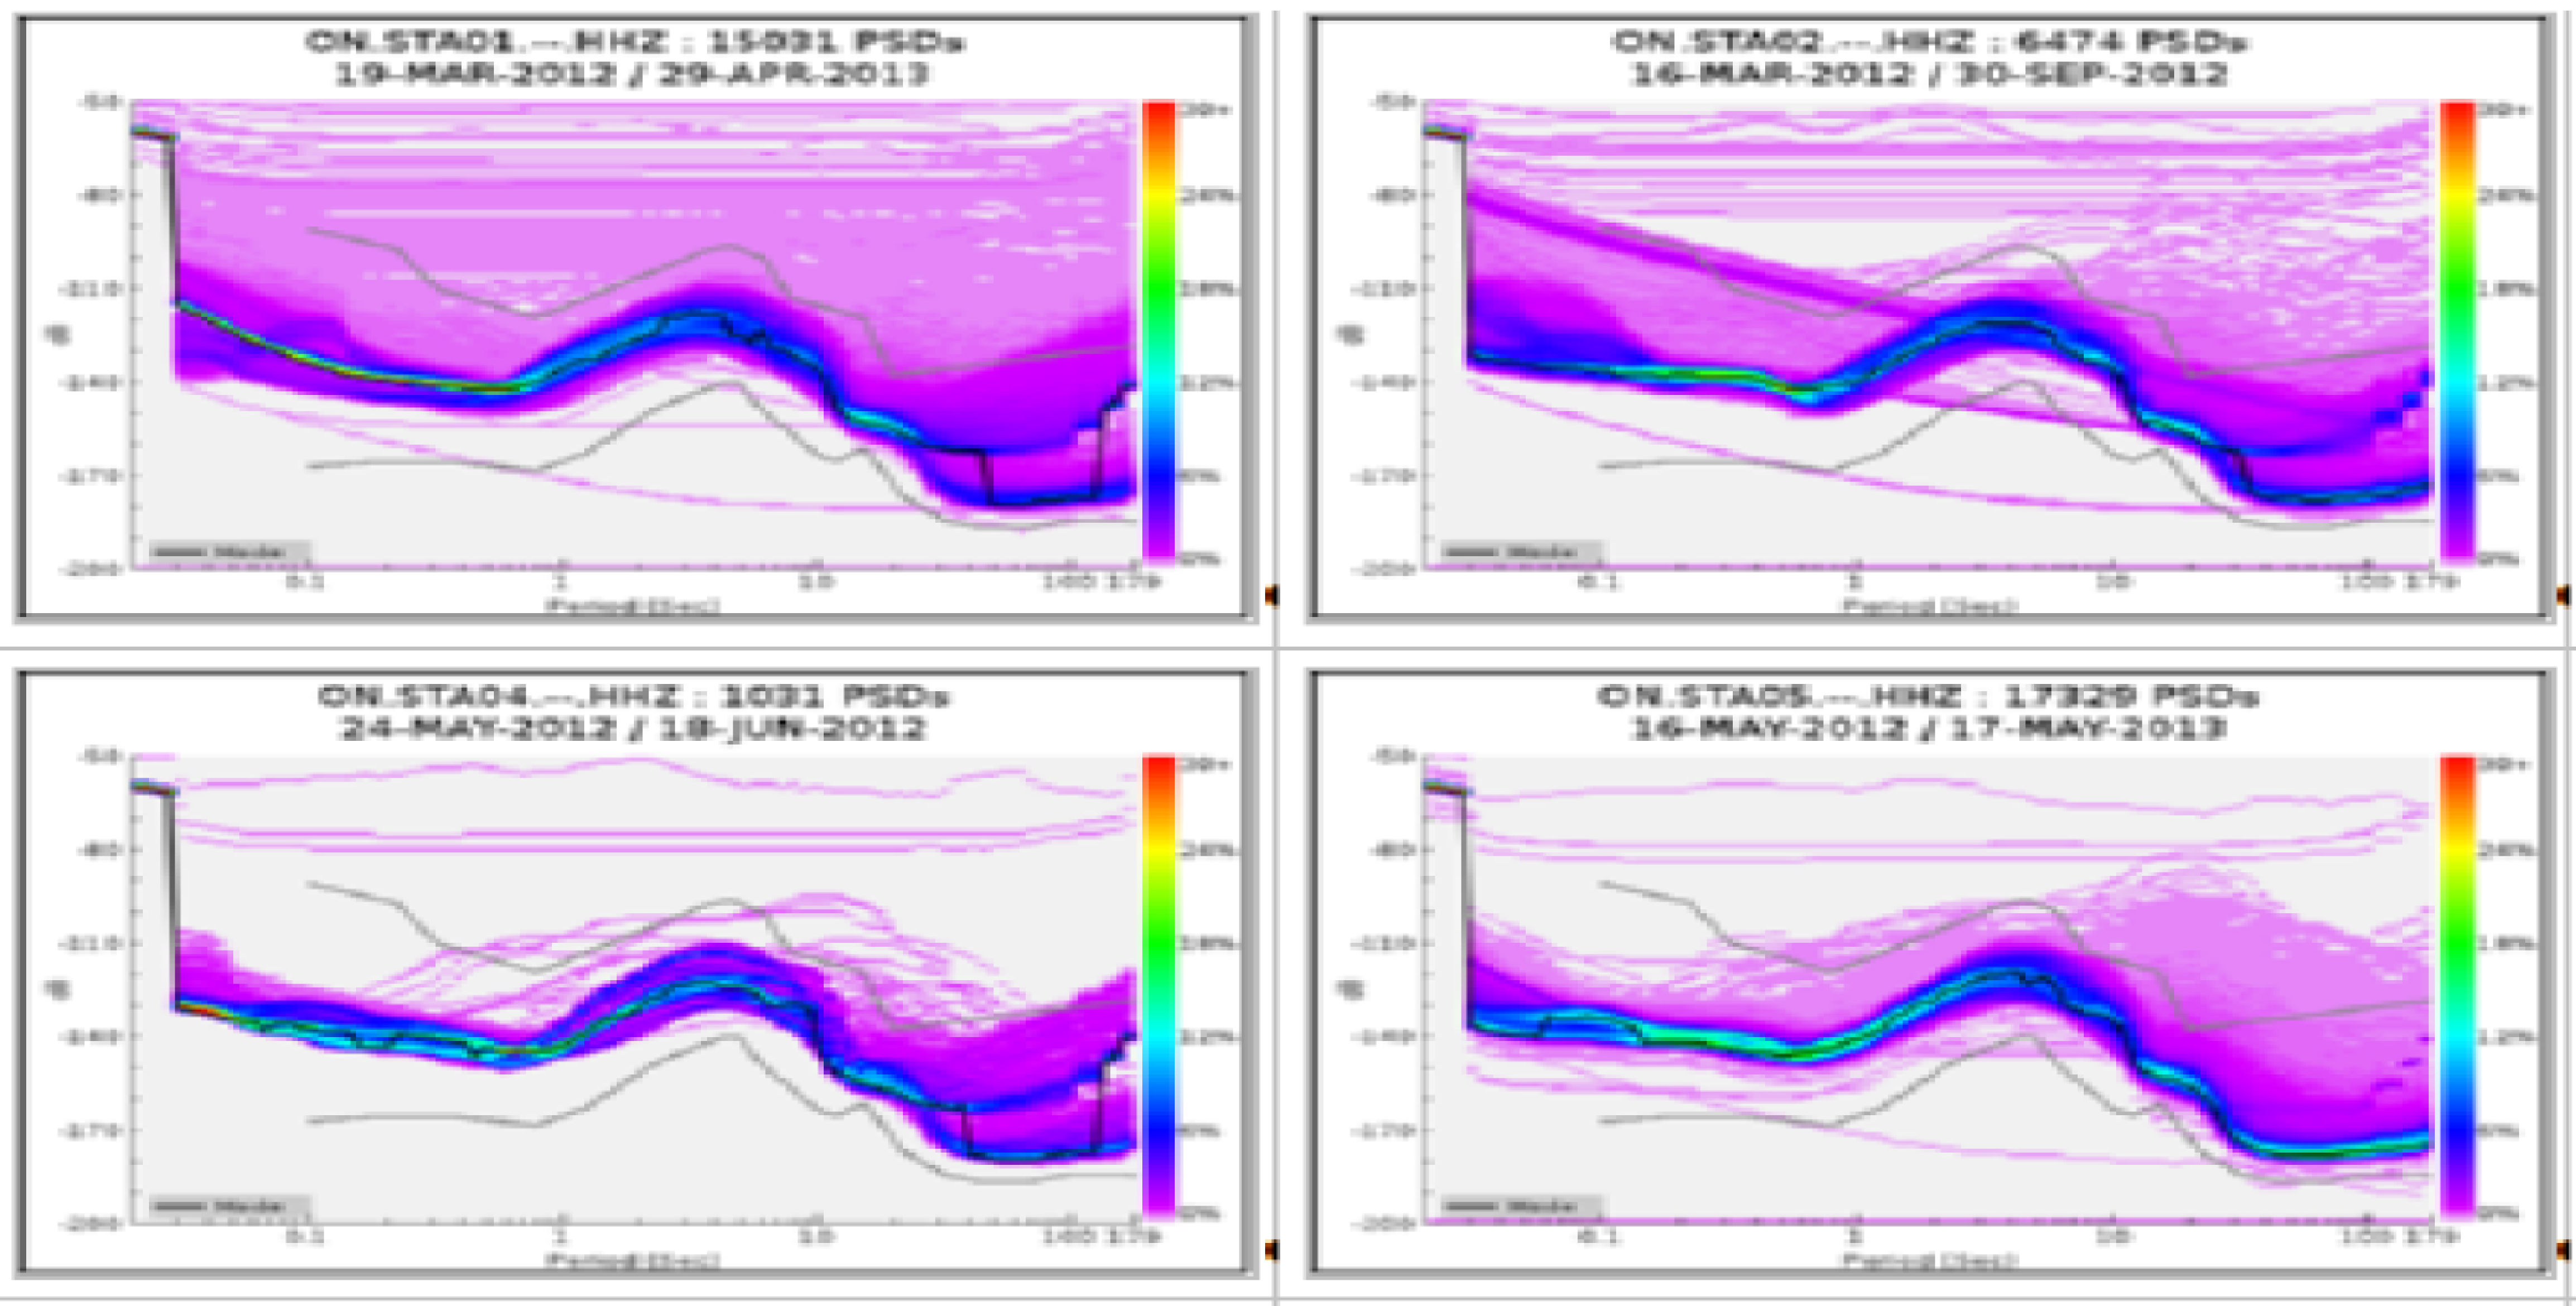
\includegraphics[scale=0.12]{exemplos_pdf.png} \caption{Examples of evaluation of data quality by the method of \cite{mcnamara_ambient_2004}} 
\label{figura4}
\end{figure}

In some stations, high probabilities appear in short and long period. This is related with diurnal variations. These changes are connected with human activity (short period) and temperature (long period). In general, the noise of short period is compound for noise generated in humans activities, with interval between 1 and 15 seconds, as shown in Figure \ref{figura4}. This noise type is dominated for micro-seisms. In noise of long period ($>$30 s) the influence of atmospheric pressure variation and temperature can alter the noise level. In case of temporary installation, the thermic isolation is basic, which carries a high level of long period noise. The quakes generate signal of high frequency (1-10 Hz), in case of local or regional seisms, already the teleseisms are of long period (10-20 seconds).

The Figure \ref{figura5} shows a section of Receiver Functions obtained from several events and normalized by the amplitude of the first peak. The first peak is the direct P-wave arrival, the second highest, around 5 seconds, is the P wave converted to S wave in the Moho discontinuity. 

\begin{figure}[!ht]
\centering
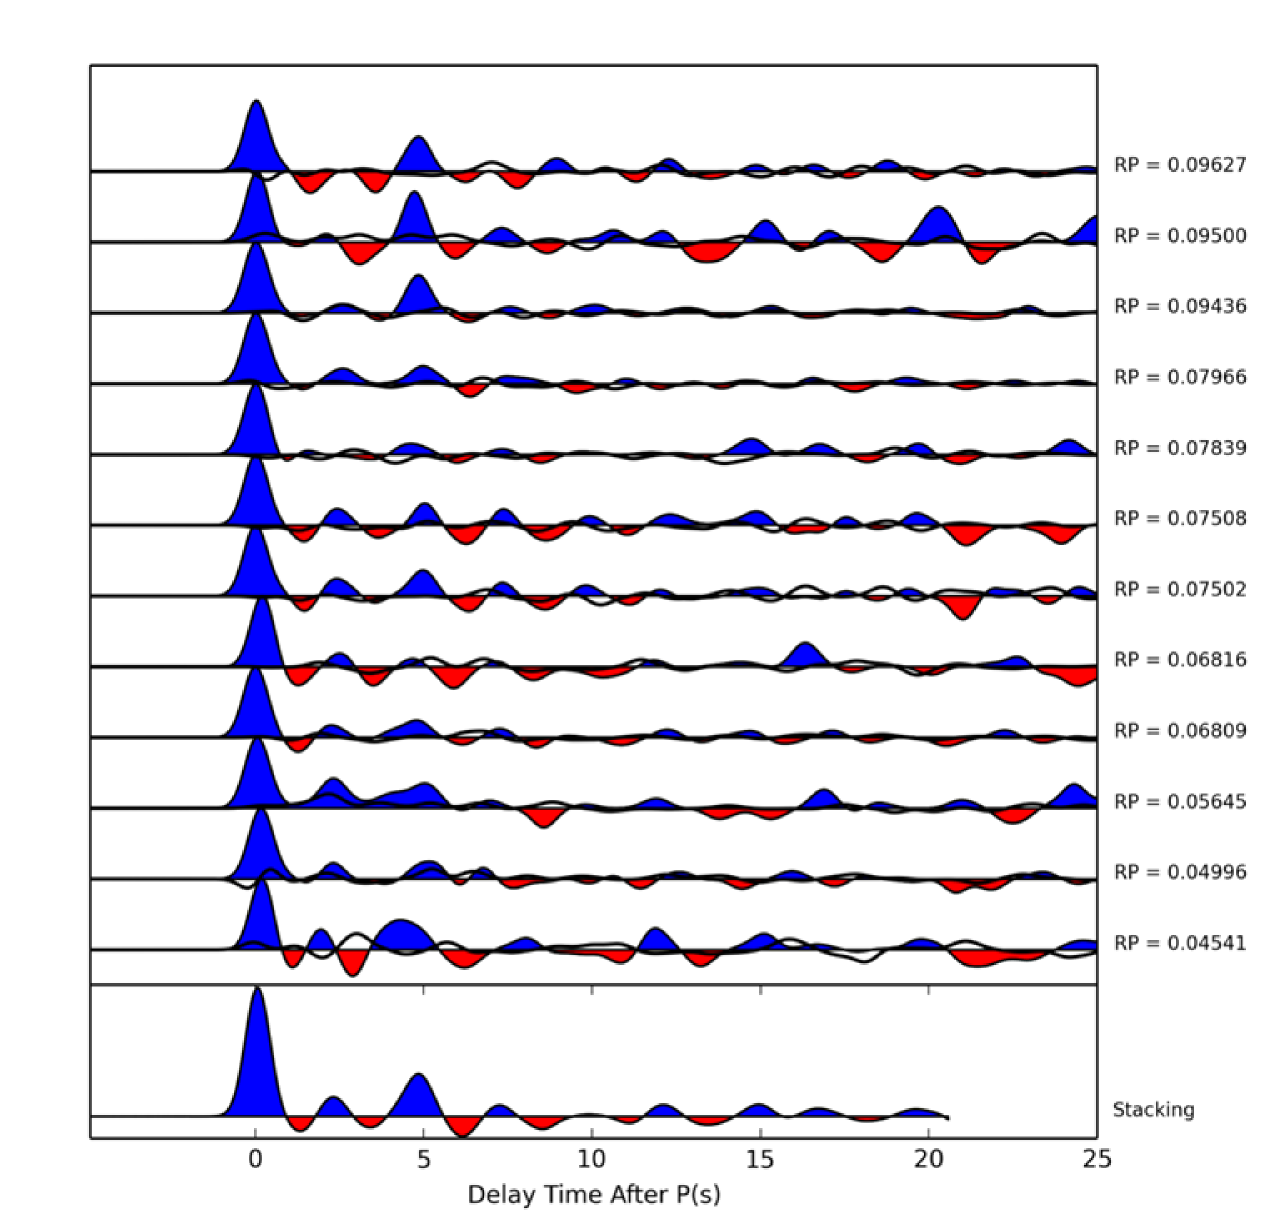
\includegraphics[scale=0.35]{funcoes_do_receptor_calculadas.png}
\caption{Receiver Functions calculated to the STA08 station and the simple stacking.}
\label{figura5}
\end{figure}

The multiples PpPs e PpSs+PsPs not have a high amplitude. The Figure \ref{figura5} shows also the deconvolution of transversal component by the vertical component.Assuming a medium, without lateral variation, the deconvolution should be zero. The small amplitude of transversal component suggests a little lateral alteration in the properties of medium. To amplify the signal-noise ratio of second peak in Receiver Functions a simple stacking of all functions was realized. After, the data separation in four groups divided by the azimuth between the quake and the station. 

We noted in Figure \ref{figura6} a substantial subsidence under the station STA04. We realized signals before the Moho, among 2 and 4 seconds, who have a depth variations along the profile. This can be related to interfaces with a contrast of different physical property. The negative pulse, red color, indicates an existence of a low-velocity layer. According with geological setting, we can infer that layer is the Taubat\`{e} basin, because this basin is located in a rift system, and this explain the subsidence of Mantle.

We calculated the crustal thickness (H) that maximizes the value of real amplitudes of Receiver Function. The best combination of crustal thickness and $v_{p}/v_{s}$ ratio calculated for each station is found in Table \ref{tabela}. The solutions found corroborate with the results from \cite{assumpcao_models_2013}, \cite{assumpcao_crustal_2013} and \cite{van_der_meijde_gravity_2013} in data of compilations from works of South America and Brazil. The obtained values for crustal thickness in Table \ref{tabela} are according with the mean measured by \cite{assumpcao_models_2013}, \cite{assumpcao_crustal_2013} and \cite{van_der_meijde_gravity_2013}, is about 30~40 km.

\begin{figure}[!ht]
\centering
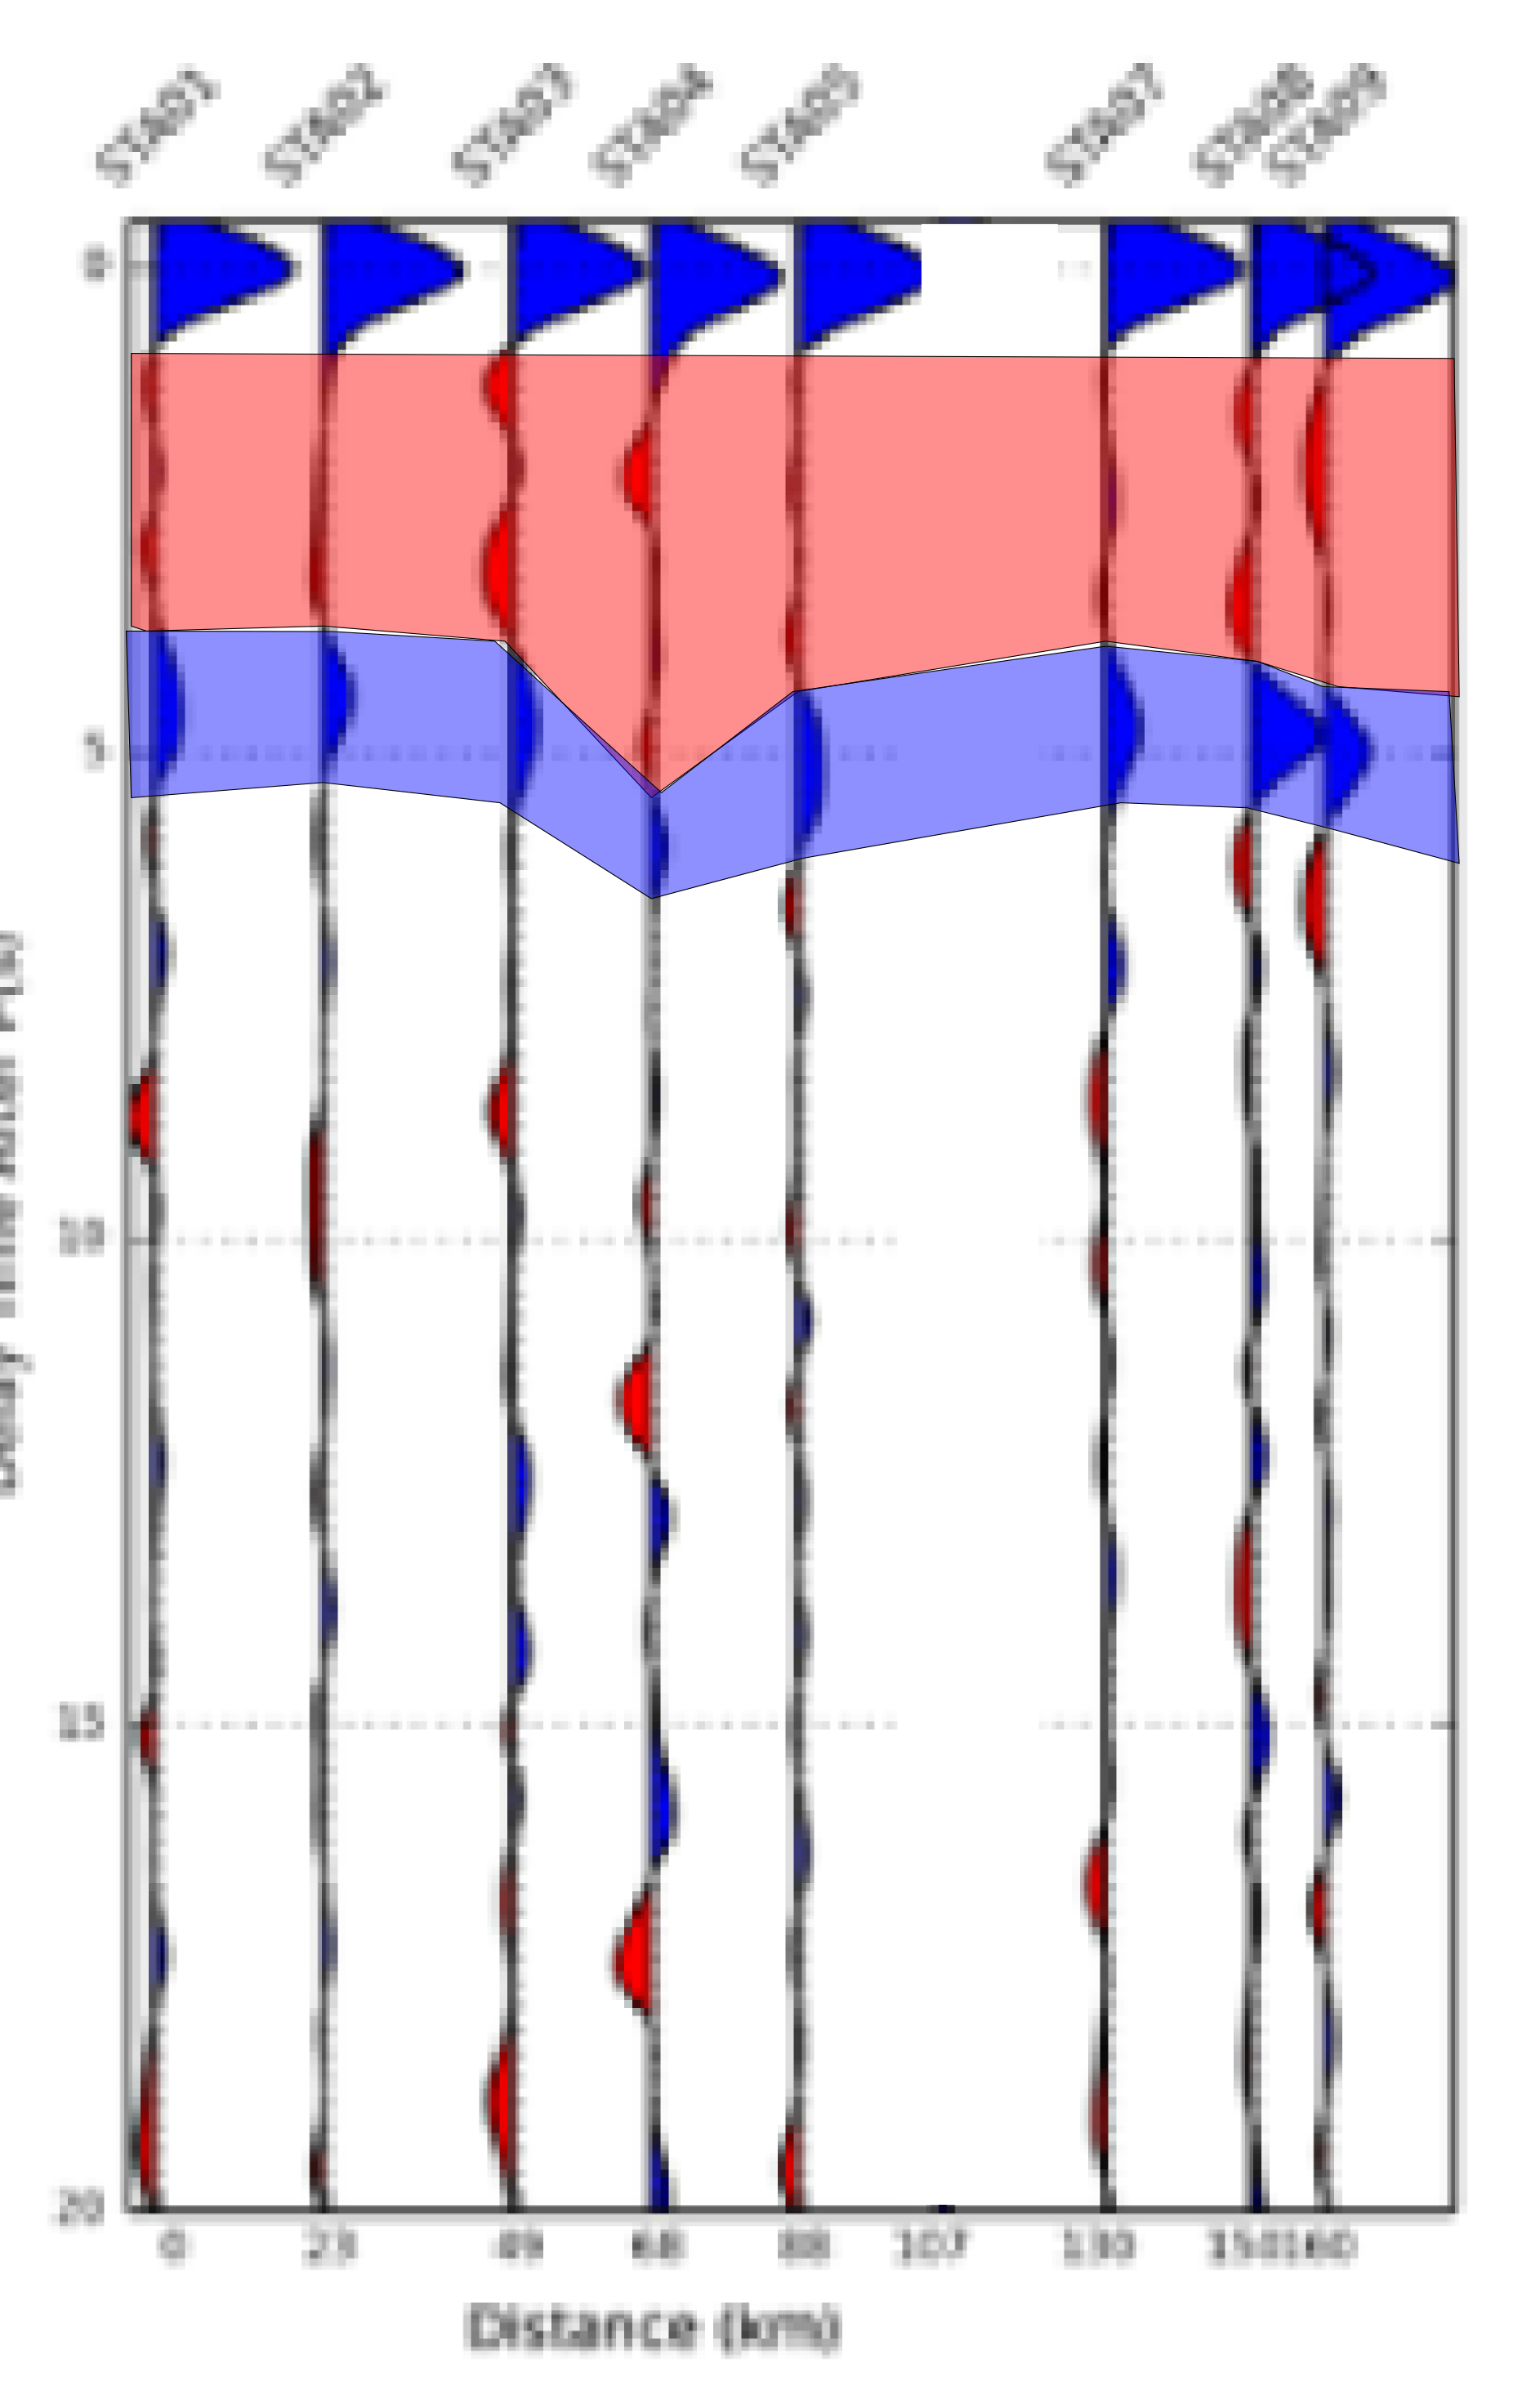
\includegraphics[scale=0.15]{empilhamento_FR_NW.png} \caption{Section of Receiver Functions} 
\label{figura6}
\end{figure}

The uncertainty, shown in Table \ref{tabela} are linked to quality and quantity of the Receiver Functions. A important phase is the selection of the best Receiver Functions, because the data quality is preponderant over the quantity. The uncertainty associated a each one of obtained parameters by the method Hk and estimated generally by "bootstrap" method, developed for  \citep{efron_statistical_1991}. From the original set of Receiver Functions the program generates subsets containing traces randomly selected. These method is repeated for each subsets, resulting in a parameter set H and $v_{p}/v_{s}$ .Mean and standard deviation from the values provide us a mean value and an estimate of the uncertainty associated to determination. There is no rule for determining the number subsets that must be generated, the crucial is search a value that makes the estimative stabilize,  including uncertainties. In general we use a value between 100 and 200 subsets depending on the amount de traces available during the “bootstrap”.

\begin{table*}[!ht]
\caption{Table with crustal thickness and $v_{p}/v_{s}$ ratio.}
\begin{center}
\begin{tabular}{| c | c | c | c | c | c | c | c | c |}
\toprule
{\textbf{Station}} & {\textbf{Altitude}} & {\textbf{Latitude}} & {\textbf{Longitude}} & {\textbf{Depth}} & {\textbf{Uncertainty}} & {\textbf{Vp/Vs ratio}} & {\textbf{Uncertainty}} & {\textbf{Number}}\\
\bottomrule
STA01 & -23.049408 & -45.016808 & 950 & 35.4000 & 3.1246 & 1.7500 & 5.96E-002 & 5\\
STA02 & -22.977707 & -45.072017 & 886 & 35.6000 & 1.5851 & 1.7200 & 4.28E-002 & 15\\
STA03 & -22.840839 & -45.194141 & 576 & 35.0000 & 8.3778 & 1.7300 & 9.84E-002 & 19\\
STA04 & -22.673525 & -45.323162 & 902 & 37.0000 & 7.2112 & 1.7400 & 1.23E-001 & 6\\
STA05 & -22.5325 & -45.432383 & 1100 & 41.0000 & 6.9241 & 1.6700 & 1.62E-001 & 29\\
STA06 & -22.386261 & -45.549086 & 931 & 55.2000 & 30.9314 & 1.7900 & 1.05E-001 & 8\\
STA07 & -22.241667 & -45.647361 & 988 & 38.8000 & 1.7971 & 1.7000 & 4.80E-002 & 24\\
STA08 & -22.050056 & -45.781374 & 884 & 33.2000 & 6.3031 & 1.8500 & 1.33E-001 & 22\\
STA09 & -21.903929 & -45.946331 & 1045 & 42.6000 & 4.3086 & 1.6800 & 8.77E-002 & 30\\
STA10 & -21.98335 & -46.29471 & 1135 & 38.8000 & 3.9148 & 1.7500 & 7.05E-002 & 5\\
STA11 & -22.12999 & -46.20536 & 1455 & 41.0000 & 4.2658 & 1.7100 & 9.04E-002 & 11\\
STA12 & -22.32379 & -46.01047 & 890 & 37.4000 & 0.6134 & 1.7700 & 1.52E-002 & 25\\
STA13 & -22.52571 & -45.86029 & 918 & 35.8000 & 3.2668 & 1.7800 & 7.67E-002 & 13\\
STA14 & -22.67147 & -45.77467 & 974 & 38.0000 & 2.9979 & 1.8000 & 7.40E-002 & 12\\
STA15 & -23.10378 & -45.39983 & 895 & 35.8000 & 0.8721 & 1.7400 & 3.26E-002 & 6\\
STA16 & -23.2387 & -45.25919 & 906 & 32.2000 & 4.1659 & 1.8000 & 1.06E-001 & 7\\
STA17 & -23.0337 & -46.62914 & 776 & 37.8000 & 1.5258 & 1.6900 & 4.39E-002 & 6\\
STA18 & -22.84539 & -46.52033 & 957 & 41.0000 & 8.0172 & 1.7200 & 1.32E-001 & 5\\
STA19 & -22.71192 & -46.27943 & 1413 & 39.0000 & 2.5130 & 1.7500 & 6.23E-002 & 18\\
STA20 & -22.56621 & -45.96951 & 908 & 38.2000 & 4.1389 & 1.7500 & 8.20E-002 & 11\\
STA21 & -22.39548 & -45.75364 & 957 & 39.0000 & 4.8590 & 1.7200 & 1.07E-001 & 9\\
\hline
\end{tabular}
\label{tabela}
\end{center}
\end{table*}

The calculated values of the Moho depth for each station were linearly interpolated to generate a regional map, shown in the Figure \ref{figura7}. To improve the interpolation, we added data from \citep{assumpcao_crustal_2013}. In the Figure \ref{figura7} we can see the Moho thinning in direction to east, reinforcing the proximity with the oceanic crust.

\begin{figure}[!ht]
\centering
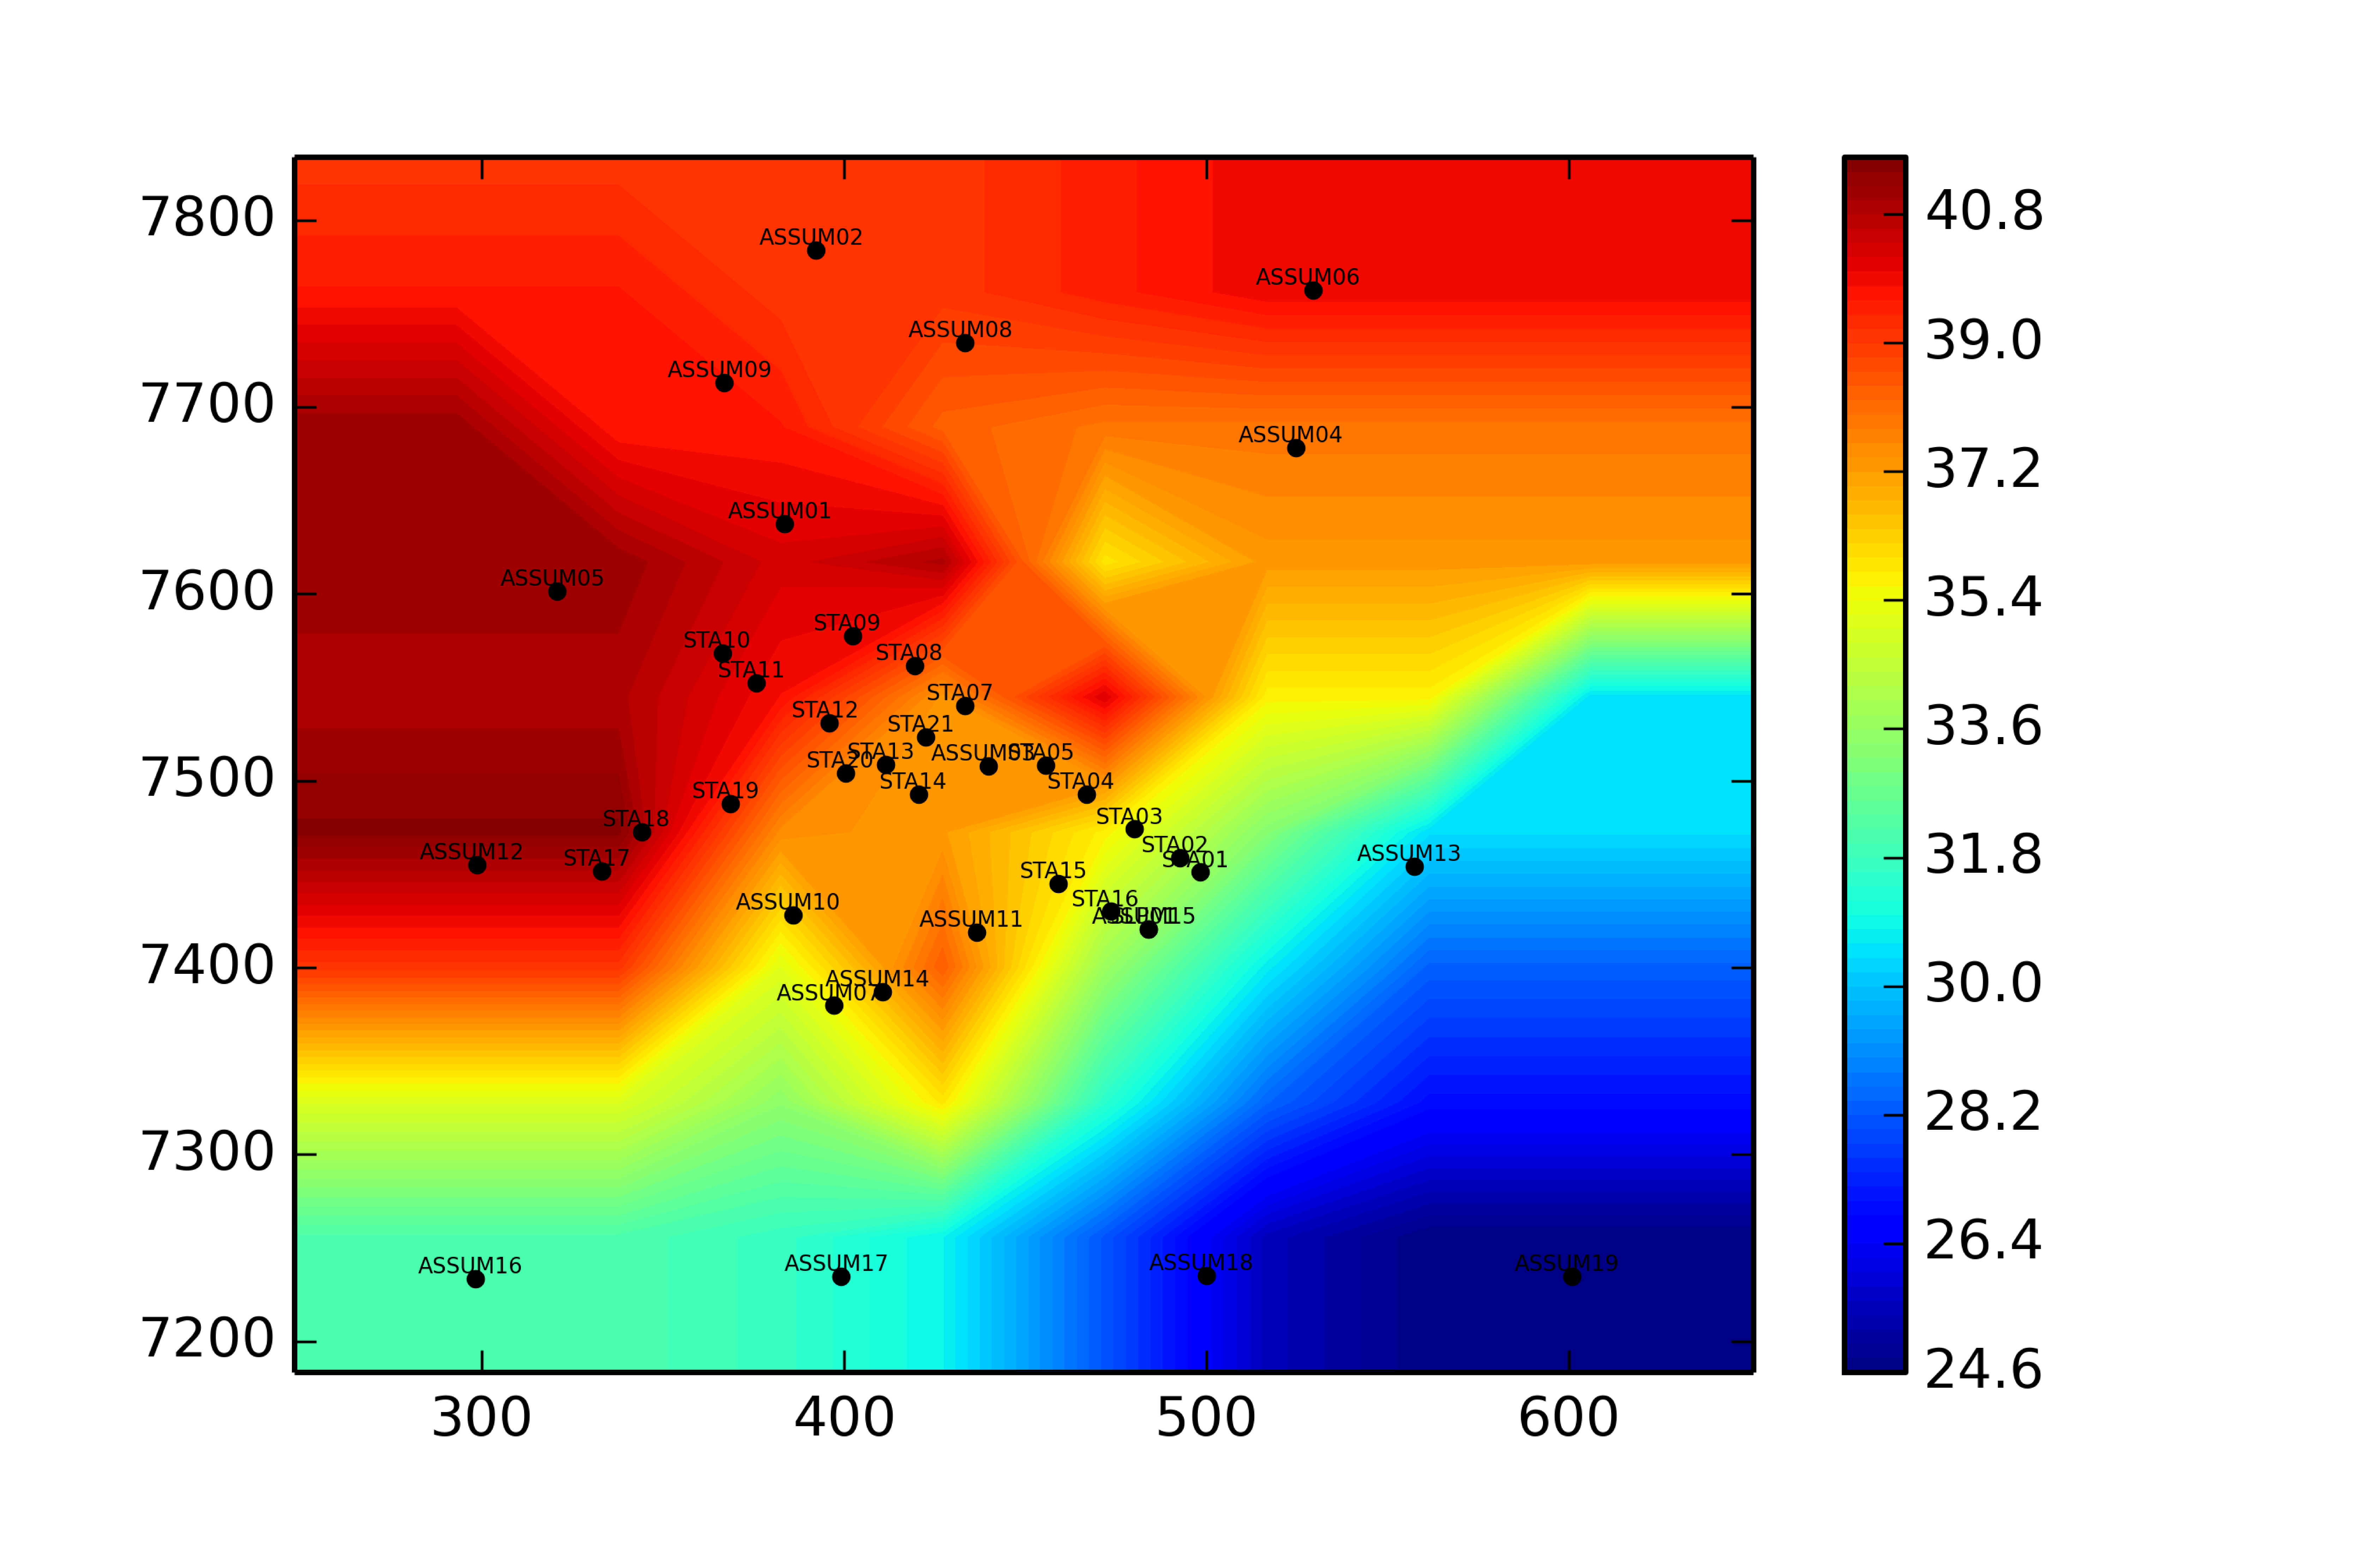
\includegraphics[scale=0.1]{Interpolacao_Linear.png} \caption{Linear Interpolation of Moho depth of each station more data from \citep{assumpcao_crustal_2013}} 
\label{figura7}
\end{figure}



\section{Conclusions}

The data analysis indicate same preliminary results about the Moho depth in the region between S\~{a}o Paulo, Minas Gerais and Rio de Janeiro. The Receiver Functions also assist to establish a image of the Crustal Framework. The generated images show a thinning trend in East direction, boundary of the continental crust.

\bibliographystyle{seg}  
\bibliography{relatorioref}


\section{Acknowledgments}

The authors wish to express their gratitude to Observat\'{o}rio Nacional and Seismographic Network for available the research data.

\end{document}


